\documentclass{beamer}

\documentclass[aspectratio=169]{beamer}

% activate me to make slides with no animation
%\documentclass[handout]{beamer}

\usepackage[warn]{mathtext}
\usepackage[T2A]{fontenc}
\usepackage[utf8]{inputenc}
\usepackage[english,russian]{babel}

\usepackage{amssymb}
\usepackage{amsmath}
\usepackage{multirow}
\usepackage{graphicx}
\usepackage{verbatim}
\usepackage{comment} 
\usepackage{pstricks}


\usepackage[cache=false]{minted}
\usepackage{listings}

\lstset{language=Java,
                basicstyle=\footnotesize\ttfamily,
                keywordstyle=\footnotesize\color{blue}\ttfamily,
}

\usepackage{adjustbox}


%%%%%%%%%%%%%%%%%%%%%%%%%%%%%%%%%  fix-lstlinebgrd.tex 
\makeatletter
\let\old@lstKV@SwitchCases\lstKV@SwitchCases
\def\lstKV@SwitchCases#1#2#3{}
\makeatother
\usepackage{lstlinebgrd}
\makeatletter
\let\lstKV@SwitchCases\old@lstKV@SwitchCases
        
\lst@Key{numbers}{none}{%
    \def\lst@PlaceNumber{\lst@linebgrd}%
    \lstKV@SwitchCases{#1}%
    {none:\\%
     left:\def\lst@PlaceNumber{\llap{\normalfont
                \lst@numberstyle{\thelstnumber}\kern\lst@numbersep}\lst@linebgrd}\\%
     right:\def\lst@PlaceNumber{\rlap{\normalfont
                \kern\linewidth \kern\lst@numbersep
                \lst@numberstyle{\thelstnumber}}\lst@linebgrd}%
    }{\PackageError{Listings}{Numbers #1 unknown}\@ehc}}
\makeatother
%%%%%%%%%%%%%%%%%%%%%%%%%%%%%%%%%


%%%%%%%%%%%%%%%%%%%%%%%%%%%%%%%%%  bListHL
\makeatletter
%%%%%%%%%%%%%%%%%%%%%%%%%%%%%%%%%%%%%%%%%%%%%%%%%%%%%%%%%%%%%%%%%%%%%%%%%%%%%%
%
% \btIfInRange{number}{range list}{TRUE}{FALSE}
%
% Test in int number <number> is element of a (comma separated) list of ranges
% (such as: {1,3-5,7,10-12,14}) and processes <TRUE> or <FALSE> respectively

\newcount\bt@rangea
\newcount\bt@rangeb

\newcommand\btIfInRange[2]{%
    \global\let\bt@inrange\@secondoftwo%
    \edef\bt@rangelist{#2}%
    \foreach \range in \bt@rangelist {%
        \afterassignment\bt@getrangeb%
        \bt@rangea=0\range\relax%
        \pgfmathtruncatemacro\result{ ( #1 >= \bt@rangea) && (#1 <= \bt@rangeb) }%
        \ifnum\result=1\relax%
            \breakforeach%
            \global\let\bt@inrange\@firstoftwo%
        \fi%
    }%
    \bt@inrange%
}
\newcommand\bt@getrangeb{%
    \@ifnextchar\relax%
        {\bt@rangeb=\bt@rangea}%
        {\@getrangeb}%
}
\def\@getrangeb-#1\relax{%
    \ifx\relax#1\relax%
        \bt@rangeb=100000%   \maxdimen is too large for pgfmath
    \else%
        \bt@rangeb=#1\relax%
    \fi%
}
%%%%%%%%%%%%%%%%%%%%%%%%%%%%%%%%%%%%%%%%%%%%%%%%%%%%%%%%%%%%%%%%%%%%%%%%%%%%%%
%
% \btLstHL<overlay spec>{range list}
%
% TODO BUG: \btLstHL commands can not yet be accumulated if more than one overlay spec match.
%
\newcommand<>{\btLstHL}[1]{%
\only#2{\btIfInRange{\value{lstnumber}}{#1}{\color{yellow}\def\lst@linebgrdcmd{\color@block}}{\def\lst@linebgrdcmd####1####2####3{}}}%
}%

\newcommand<>{\btLstHLG}[1]{%
\only#2{\btIfInRange{\value{lstnumber}}{#1}{\color{green}\def\lst@linebgrdcmd{\color@block}}{\def\lst@linebgrdcmd####1####2####3{}}}%
}%
\makeatother
%%%%%%%%%%%%%%%%%%%%%%%%%%%%%%%%%

\newcommand{\showTOC}{
    \begin{frame}[noframenumbering,plain]
        \frametitle{Вы находитесь здесь}
        \tableofcontents[currentsection]
    \end{frame}
}



\title[Concurrency: VM engineer point of view]{!concurrent,worldHello\\ или \\ многопоточность глазами VM-инженера}
\author[Александр Филатов]{Александр Филатов\\ filatovaur@gmail.com\\ {\tiny\url{https://github.com/Svazars/snowone-2024-vm-engineer-concurrency}}}

\date{}

\usetheme{CambridgeUS}

% tikz
\usepackage{pgf}
\usepackage{tikz}
\usepackage{tikz-qtree}
\usetikzlibrary{arrows, automata, fit, shapes, shapes.multipart, trees, positioning}

\usepackage{array}
\usepackage{cancel}
\usepackage{hyperref}
\usepackage[normalem]{ulem}

\begin{document}


% tikz common
\newcommand{\uedge}[2]{(#1) edge node {} (#2)}
\newcommand{\cedge}[3]{(#1) edge[#3, line width=1mm] node {} (#2)}
\newcommand{\cedgel}[3]{(#1) edge[#3, line width=0.5mm] node {} (#2)}
\newcommand{\nodesize}{1cm}

\begin{frame}
  \titlepage
\end{frame}

\section{Знакомство}

\begin{frame}{Bio: Александр Филатов}

Уже 8 лет как VM-инженер\footnote{\tiny Иван Углянский, Один день из жизни JVM-инженера, \url{https://habr.com/ru/company/jugru/blog/719614/}}

\begin{itemize}
    \item 2015 - 2019, Excelsior JVM with AOT compilation\footnote{\tiny\url{https://habr.com/ru/company/jugru/blog/437180/}}
    \item 2019 - now, Huawei, Languages and Compilers lab\footnote{\tiny\url{http://rnew.tilda.ws/excelsiorathuawei}}
\end{itemize}

\pause

Специализация -- рантаймы виртуальных машин

Узкая специализация -- сборщики мусора

\end{frame}

\begin{frame}{Bio: Александр Филатов}

Область интересов: 

\begin{itemize}
 \item автоматическое управление памятью

 \pause
 \item многопоточность

 \pause
 \item слабые модели памяти

 \pause
 \item корректность многопоточных структур данных
\end{itemize}


\pause
Персональное когнитивное искажение: много страдал, отлаживая баги 
\begin{itemize}
 \item своего параллельного кода

 \pause
 \item чужих реализаций многопоточных структур данных

 \pause
 \item компилятора
\end{itemize}

\pause
Опасаюсь нового. Не люблю поддерживать старое.

\end{frame}

\begin{frame}[t,fragile]{Как было получено название доклада}
\framesubtitle{!concurrent,worldHello}

\begin{minted}[fontsize=\small]{java}
 for (String msg : new String[] {
       "Hello", ",", "concurrent", "world", "!"
    }) {
    new Thread() {
        public void run() {
            System.out.println(msg);
        }
    }.start();
 }
 \end{minted}

\pause


\begin{tikzpicture}[remember picture,overlay]
\node[xshift=3cm,yshift=-2.0cm] at (current page.center) {
\includegraphics[width=.6\textwidth]{production/scaried-guys.png}};
\end{tikzpicture}


\end{frame}


\begin{frame}{План выступления}
\tableofcontents
\end{frame}



\section{Как я вижу программистов}
\showTOC


\begin{frame}[t,fragile]{Идея №1: давай распараллелим!}
\framesubtitle{Обычно бывает так}

Коллега предлагает переписать часть проекта с использованием нескольких потоков

\end{frame}


\begin{frame}[t,fragile,noframenumbering]{Идея №1: давай распараллелим!}
\framesubtitle{Обычно бывает так}

Коллега предлагает переписать часть проекта с использованием нескольких потоков

\begin{tikzpicture}[remember picture,overlay]
\node[xshift=3cm,yshift=-1.5cm] at (current page.center) {
\includegraphics[width=.3\textwidth]{production/fry-easy.jpg}};
\end{tikzpicture}

\pause

Проходит время ...

\pause

\begin{itemize}
  \item Стало медленнее
  \pause
  \item Зависает
\end{itemize}

\end{frame}


 \begin{frame}[t,fragile,noframenumbering]{Идея №1: давай распараллелим!}
 \framesubtitle{Обычно бывает так}
 
 Коллега предлагает переписать часть проекта с использованием нескольких потоков
 
 \begin{tikzpicture}[remember picture,overlay]
 \node[xshift=3cm,yshift=-4.35cm] at (current page.center) {
\includegraphics[width=.3\textwidth]{production/fry-easy.jpg}};
 \end{tikzpicture}
 
 Проходит время ...
 
 \begin{itemize}
   \item Стало медленнее
   \item Зависает
   \item Код непонятный
 \end{itemize}
 
 \end{frame}


\begin{frame}[t,fragile,noframenumbering]{Идея №1: давай распараллелим!}
\framesubtitle{Обычно бывает так}

Коллега предлагает переписать часть проекта с использованием нескольких потоков

\begin{tikzpicture}[remember picture,overlay]
\node[xshift=3cm,yshift=-4.0cm] at (current page.center) {
\includegraphics[width=.2\textwidth]{production/devil-latest.png}};
\end{tikzpicture}


Проходит время ...

\begin{itemize}
  \item Стало медленнее
  \item Зависает
  \item Код непонятный
\end{itemize}

\end{frame}


\begin{frame}[t,fragile]{Идея №1: давай распараллелим!}
\framesubtitle{Почему так происходит?}

\pause

 \begin{tabular}{p{0.5\textwidth} p{0.5\textwidth}}
 \begin{minted}[fontsize=\small]{java}
 synchronized(objectA) {
  synchronized(objectB) {
    computeStuff();
  }
 }
 \end{minted}
 
 & 
 
 \begin{minted}[fontsize=\small]{java}
 synchronized(objectB) {
  synchronized(objectA) {
    computeStuff();
  }
 }
 \end{minted}
 \end{tabular}

\pause 
Легко сломать многопоточную систему неаккуратным изменением.

\pause
Это ВСЕГДА случается после написания оригинального кода.

\pause

\begin{tikzpicture}[remember picture,overlay]
\node[xshift=-4cm,yshift=-6.0cm] at (current page.center) {
\includegraphics[width=.4\textwidth]{production/kiss/kiss.png}};
\node[xshift=3cm,yshift=-6.0cm] at (current page.center) {
\includegraphics[width=.35\textwidth]{production/kiss/1-prof-kiss.jpg}};
\end{tikzpicture}

\end{frame}


\begin{frame}[t]{Идея №1: давай распараллелим!}
\framesubtitle{Выводы}

Параллелизм полезен, но многопоточность приносит с собой:
\begin{itemize}
  \item Риски
  \item Издержки на поддержку
\end{itemize}

\pause
Реакция VM-инженера: изыди! Не хочу отлаживать этот код через полгода, после серии несвязанных правок, когда ты уже уволишься.

\pause
Реакция здорового человека: давай подумаем, стоит ли оно того.

\end{frame}


\begin{frame}[t]{Идея №2: давай по книжке сделаем!}
\framesubtitle{Взгляд VM-инженера}

\begin{tabular}{p{0.5\textwidth} p{0.5\textwidth}}  
\centering{Реальность} & 
\end{tabular}

\begin{tikzpicture}[remember picture,overlay]
\node[xshift=-3.2cm,yshift=-7.5cm] at (current page.center) {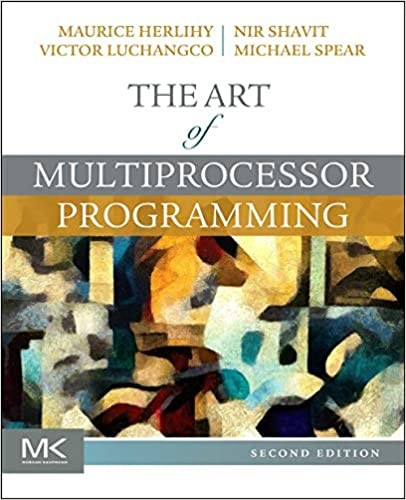
\includegraphics[width=.35\textwidth]{production/art-cover.jpg}};
\end{tikzpicture}

\end{frame}


\begin{frame}[t,noframenumbering]{Идея №2: давай по книжке сделаем!}
\framesubtitle{Взгляд VM-инженера}

\begin{tabular}{p{0.5\textwidth} p{0.5\textwidth}}  
\centering{Реальность} & \centering{Мои ощущения}
\end{tabular}

\begin{tikzpicture}[remember picture,overlay]
\node[xshift=-3.2cm,yshift=-7.5cm] at (current page.center) {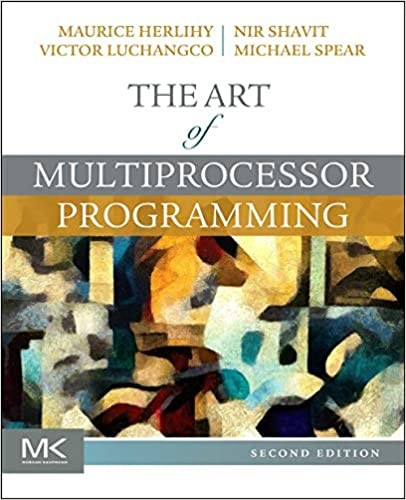
\includegraphics[width=.35\textwidth]{production/art-cover.jpg}};
\end{tikzpicture}

\begin{tikzpicture}[remember picture,overlay]
\node[xshift=3.2cm,yshift=-7cm] at (current page.center) {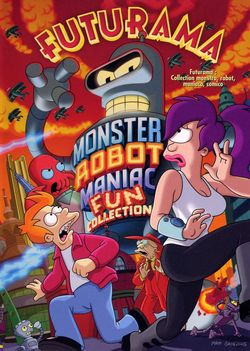
\includegraphics[width=.3\textwidth]{production/maniac-book.png}};
\end{tikzpicture}

\end{frame}


\begin{frame}[t]{Идея №2: давай по книжке сделаем!}
\framesubtitle{KSUH lock}

“A Fair Fast Scalable Reader-Writer Lock “, 1993

\begin{itemize}
  \item Orran \textbf{K}rieger, Michael \textbf{S}tumm, Ron \textbf{U}nrau, Jonathan \textbf{H}anna
  \item In Proc. of the International Conference on Parallel Processing

  \pause
  \item реализовано на языке Си

  \pause
  \item алгоритм формализован на языке Promela и верифицирован инструментом SPIN % TODO-link, TODO-footnote верифицирован частично

\end{itemize}

\pause

“Using Hardware Transactional Memory to Correct and Simplify and Readers-writer Lock Algorithm”, 2013
\begin{itemize}

  \pause
  \item 20 лет спустя!

  \pause
  \item Обнаружена ошибка в алгоритме, связанная с управлением памятью. Проявлялась на реальной системе.
\end{itemize}

\end{frame}


\begin{frame}[t,noframenumbering]{Идея №2: давай по книжке сделаем!}
\framesubtitle{KSUH lock}

“A Fair Fast Scalable Reader-Writer Lock “, 1993

\begin{itemize}
  \item Orran \textbf{K}rieger, Michael \textbf{S}tumm, Ron \textbf{U}nrau, Jonathan \textbf{H}anna
  \item In Proc. of the International Conference on Parallel Processing
  \item реализовано на языке Си
  \item алгоритм формализован на языке Promela и \textbf{верифицирован}\footnote{частично} инструментом SPIN
\end{itemize}

“Using Hardware Transactional Memory to Correct and Simplify and Readers-writer Lock Algorithm”, 2013
\begin{itemize}
  \item 20 лет спустя!
  \item Обнаружена ошибка в алгоритме, связанная с управлением памятью. Проявлялась на реальной системе.
\end{itemize}

\end{frame}


\begin{frame}[t]{Идея №2: давай по книжке сделаем!}
\framesubtitle{Выводы}

Сложные алгоритмы нужны, но приносят с собой:
\begin{itemize}
  \item Риски
  \item Издержки на поддержку
\end{itemize}


\pause
Реакция VM-инженера: ты точно понимаешь, что написано в книжке и почему оно будет работать?

\pause
Реакция здорового человека: неудобно, если для редактирования кода требуется кандидатская степень по распределенным системам. 

\pause

\includegraphics[width=.3\textwidth]{production/kiss/2-bender-kiss.png}


\begin{tikzpicture}[remember picture,overlay]
\node[xshift=2cm,yshift=-2.5cm] at (current page.center) {
\includegraphics[width=.4\textwidth]{production/kiss/kiss.png}};
\end{tikzpicture}

\end{frame}


\begin{frame}[t]{Идея №2: давай по книжке сделаем!}
\framesubtitle{Но если ты эксперт, то тогда можно?}

Промышленные системы быстры благодаря хитрым решениям.

\pause

\includegraphics[width=.3\textwidth]{production/super-duper.png}

\pause

\begin{tikzpicture}[remember picture,overlay]
\node[xshift=1.5cm,yshift=-1.5cm] at (current page.center) {
\includegraphics[width=.4\textwidth]{production/morbo.png}};
\end{tikzpicture}

\end{frame}


\begin{frame}[t,noframenumbering,fragile]{Идея №2: давай по книжке сделаем!}
\framesubtitle{Но если ты эксперт, то тогда можно?}

Промышленные системы быстры благодаря хитрым решениям.

Пример из Java-мира: biased locking.

\pause
Хитрая штука, чтобы ваши \textittt{synchronized} работали очень быстро\footnote<2->{\tiny\url{https://mechanical-sympathy.blogspot.com/2011/11/biased-locking-osr-and-benchmarking-fun.html}}.

\begin{minted}[fontsize=\small]{java}
while (0 != count--) {
  synchronized (jvmLock) {
    ++counter;
  }
}
\end{minted}

\pause
\begin{center}
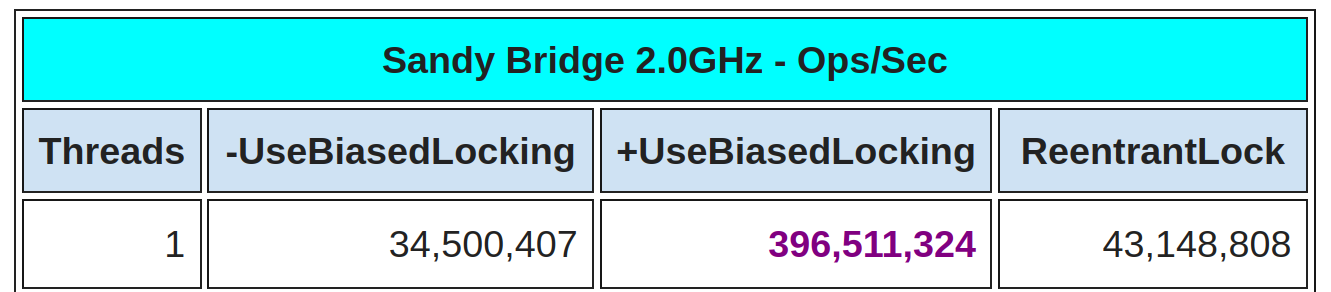
\includegraphics[width=.8\textwidth]{production/biased-locking.png}
\end{center}

\end{frame}


\begin{frame}[t,noframenumbering]{Идея №2: давай по книжке сделаем!}
\framesubtitle{Но если ты эксперт, то тогда можно?}

Промышленные системы быстры благодаря хитрым решениям.

Пример из Java-мира: biased locking.

\begin{itemize}
 \item Опубликован в 2006 году\footnote{\tiny\url{https://dl.acm.org/doi/10.1145/1167473.1167496}}

 \pause
 \item Служил верой и правдой

 \pause
 \item "Costly to maintain"

 \pause
 \item Deprecated в Java 15 (JEP 374, 2019)

\end{itemize}

\pause

\begin{tikzpicture}[remember picture,overlay]
\node[xshift=3.5cm,yshift=-5.5cm] at (current page.center) {
\includegraphics[width=.5\textwidth]{production/toad.jpeg}};
\end{tikzpicture}

\begin{tikzpicture}[remember picture,overlay]
\node[xshift=-3.5cm,yshift=-5.5cm] at (current page.center) {
\includegraphics[width=.4\textwidth]{production/kiss/kiss.png}};
\end{tikzpicture}

\end{frame}


\begin{frame}[t]{Идея №3: давай возьмем готовое!}
\framesubtitle{Хоть кто-то в состоянии написать сложную систему безошибочно?}

\pause 

\textttt{Linux futex\_wait() bug}\footnote<2->{\tiny\url{https://groups.google.com/g/mechanical-sympathy/c/QbmpZxp6C64/m/BonaHiVbEmsJ}}

\pause
Gil Tene (CEO of Azul, co-author of C4 GC):

\begin{quote}
  We had this one bite us hard and scare the \%\$\^\! out of us, so I figured I'd share the fear.
\end{quote}

\pause

\begin{quote}
The linux futex\_wait call has been broken for about a year.
\end{quote}

\pause

\begin{quote}
The impact of this kernel bug is very simple: user processes can deadlock and hang in seemingly impossible situations. Thread.park() in Java may stay parked.
\end{quote}

\pause

\begin{quote}
You'll spend a couple of months of someone's time trying to find the fault in your code, when there is nothing there to find. 
\end{quote}

\end{frame}


\begin{frame}[t,noframenumbering]{Идея №3: давай возьмем готовое!}
\framesubtitle{Хоть кто-то в состоянии написать сложную систему безошибочно?}

\begin{center}

\includegraphics[width=0.7\textwidth]{production/doom.jpg}
\end{center}

\end{frame}


\begin{frame}[t]{Идея №3: давай возьмем готовое!}
\framesubtitle{Выводы}

\begin{itemize}
  \item Выбирайте проверенные технологии
  \pause
  \item Регулярно обновляйтесь
  \pause
  \item Можете не использовать хитрые алгоритмы -- не используйте
\end{itemize}

\pause

\begin{center}

\includegraphics[width=.7\textwidth]{production/kiss/3-bart-kiss.jpg}
\end{center}

\end{frame}


% \begin{frame}{Идея №3: давай возьмем готовое!}
% 
% Василий прелагает взять библиотеку из репозитория со 100500 звездочек.
% Сотни опытнейших людей со всего мира обязательно вычитывают каждый коммит, и для нас сойдет.
% 
% Очки рантайма:
% Там import другим кеглем. Ну-ка
% Ага, import com.highway.to.hell
% 
% \end{frame}
% 
% 
% \begin{frame}{Идея №3: давай возьмем готовое!}
% 
% Пользоваться готовым надо уметь, в том числе читать непростые доки
% (MPSC не так использован, да еще присыпан неверным интерфейсом)
% 
% \end{frame}
% 
% \begin{frame}{Идея \#3: возьмем готовое!}
% 
% Ну, даже в стандартной библиотеке для Java есть "особенности"
% https://bugs.openjdk.org/browse/JDK-8256833
% [concurrency-interest] ConcurrentLinkedDeque is non-linearizable
% 
% В целом, надо думать всегда. Иногда "минимальный объем думания" для написания нормального кода весьма большой.
% 
% \end{frame}


\begin{frame}[t]{Как страшно жить}

\begin{center}
Жизнерадостный коллега 


\includegraphics[width=.4\textwidth]{production/sad-fry.png}

Почему так?

\end{center}
\end{frame}

\begin{frame}[t]{Почему так?}
\framesubtitle{Личный опыт}

Человеческий мозг не предназначен для многопоточности. 

\pause

Сложно представлять одновременное исполнение потоков и все возможные пересечения.

\pause

\begin{center}

\includegraphics[width=.6\textwidth]{production/crazy-prof.png}
\end{center}

\end{frame}
 
\begin{frame}[t]{Неконкретные советы}

Используйте
\begin{itemize}
  \item Простые решения

  \pause
  \item Готовые библиотеки для сложных стандартных задач

  \pause
  \item Шаблоны проектирования многопоточных систем

  \pause
  \item Предметно-ориентированные языки
\end{itemize}

\pause
\
\
\
\
\
\

А если меня беспокоит производительность?

\begin{tikzpicture}[remember picture,overlay]
\node[xshift=4.0cm,yshift=-5.5cm] at (current page.center) {
\includegraphics[width=.6\textwidth]{production/what-about-perf-2.png}};
\end{tikzpicture}

\end{frame}
  


\section{Как я вижу системных программистов}
\showTOC



\begin{frame}[fragile]{Ленивая инициализация}
\framesubtitle{Простой случай}

% \begin{lstlisting}[basicstyle=\fontsize{8}{8}\selectfont\ttfamily,
%     linebackgroundwidth = 17 em
% ]
\begin{minted}[fontsize=\small]{java}
public class LazyInit { 

  private Object heavyToInitialize = null;

  /**
    * Initializes resource lazily, on first `getResource`. 
    * `init` should be invoked only once.
  */
  Object getResource() {
    if (heavyToInitialize == null) {
      heavyToInitialize = init();
    }
    return heavyToInitialize;
  }
}
\end{minted}
%\end{lstlisting}
\end{frame}

\begin{frame}[fragile]{Ленивая инициализация}
\framesubtitle{Многопоточность}

\begin{lstlisting}[basicstyle=\fontsize{8}{8}\selectfont\ttfamily,
    linebackgroundwidth = 17 em
]
    private Object heavyToInitialize;
\end{lstlisting}


\begin{tabular}{p{3.5cm}p{5cm}}

\begin{lstlisting}[basicstyle=\fontsize{8}{8}\selectfont\ttfamily,
    linebackgroundwidth = 20 em,
    linebackgroundcolor={%
      \btLstHL<2-3>{2}
      \btLstHL<4-5>{3}
      \btLstHL<6-7>{4}  
      \btLstHL<8>{5}  
      \btLstHL<9->{7}  
}]
    // thread 1
    Object getResource() {
      if (heavyToInitialize == null) {

        heavyToInitialize = init();
      }
      return heavyToInitialize;
    }
\end{lstlisting}
          &
% \onslide<9->{поток №1 получил один экземпляр}
          \\


% \onslide<11->{поток №2 получил другой экземпляр}
          & 
\begin{lstlisting}[basicstyle=\fontsize{8}{8}\selectfont\ttfamily,
    linebackgroundwidth = 22 em,
    linebackgroundcolor={%
      \btLstHLG<3-4>{2}
      \btLstHLG<5-6>{3}
      \btLstHLG<7-9>{4}
      \btLstHLG<10>{5}
      \btLstHLG<11->{7}
}]
    // thread 2
    Object getResource() {
      if (heavyToInitialize == null) {
  
        heavyToInitialize = init();
      }
      return heavyToInitialize;
    }
\end{lstlisting} 
\end{tabular}

\end{frame}




\begin{frame}[fragile]{Многопоточная ленивая инициализация}
\framesubtitle{Double checked locking}

\begin{minted}[fontsize=\small]{java}
private volatile Object heavyToInitialize = null;
Object getResource() {
  if (heavyToInitialize == null) {
    synchronized(this) {
      if (heavyToInitialize == null) {
        heavyToInitialize = init();
      }
    }
  }
  return heavyToInitialize;
}
\end{minted}

\pause

\begin{tikzpicture}[remember picture,overlay]
\node[xshift=-5.0cm,yshift=-4.0cm] at (current page.center) {
\includegraphics[width=.3\textwidth]{production/fry-pain-head.png}};
\end{tikzpicture}

\pause

\begin{tikzpicture}[remember picture,overlay]
\node[xshift=4.0cm,yshift=-3.5cm] at (current page.center) {
\includegraphics[width=.5\textwidth]{production/what-about-perf-2.png}};
\end{tikzpicture}

\end{frame}


\begin{frame}{Многопоточная ленивая инициализация}
\framesubtitle{А почему так медленно?}

\begin{itemize}

\item Приходит системный программист.

\pause

\item Смотрит на реализацию стандартного шаблона программирования.

\pause

\item Считает, что можно лучше.
\end{itemize}

\end{frame}


\begin{frame}[fragile]{Многопоточная ленивая инициализация}
\framesubtitle{Trampolines: idea}

\begin{minted}[fontsize=\small]{c}
void* getResource() {
  if (heavyToInitialize == NULL) {
    heavyToInitialize = create();
  }
  return heavyToInitialize;
}
\end{minted}

\pause

\begin{minted}[fontsize=\small]{gas}
getResource: mov     rax, qword ptr [heavyToInitialize]
             test    rax, rax
             je      .LBB0_1
             ret
.LBB0_1:     ...
             call    create
             mov     qword ptr [heavyToInitialize], rax
             ...
\end{minted}

\pause

Когда инициализация завершилась, не нужно проверять rax на NULL.

\end{frame}


\begin{frame}[fragile]{Многопоточная ленивая инициализация}
\framesubtitle{Trampolines}

До инициализации:
\begin{minted}[fontsize=\small]{gas}
getResource: mov     rax, qword ptr [heavyToInitialize]
             test    rax, rax
             je      .LBB0_1
             ret
.LBB0_1:     ...
             call    create
             mov     qword ptr [heavyToInitialize], rax
             ...
\end{minted}
\end{frame}


\begin{frame}[fragile,noframenumbering]{Многопоточная ленивая инициализация}
\framesubtitle{Trampolines}

Когда проинициализировали, требуется замена выделенного участка:
\begin{minted}[fontsize=\small]{gas}
getResource: mov     rax, qword ptr [heavyToInitialize]
             test    rax, rax ; <<    
             je      .LBB0_1  ; <<    
             ret              ; <<    
.LBB0_1:     ...
             call    create
             mov     qword ptr [heavyToInitialize], rax
             ...
\end{minted}
\end{frame}

\begin{frame}[fragile,noframenumbering]{Многопоточная ленивая инициализация}
\framesubtitle{Trampolines}

После инициализации:
\begin{minted}[fontsize=\small]{gas}
getResource: mov     rax, qword ptr [heavyToInitialize]
             ret  ; test    rax, rax
             nop  ; je      .LBB0_1
             nop  ; ret
.LBB0_1:     ...
             call    create
             mov     qword ptr [heavyToInitialize], rax
             ...
\end{minted}
\end{frame}


\begin{frame}[t]{Многопоточная ленивая инициализация}
\framesubtitle{Trampolines: use cases}

Очень элегантное и производительное решение. 

\pause

\begin{tikzpicture}[remember picture,overlay]
\node[xshift=-5.0cm,yshift=-9.0cm] at (current page.center) {
\includegraphics[width=.3\textwidth]{production/fry-pain-head.png}};
\end{tikzpicture}

\end{frame}


\begin{frame}[t]{Многопоточная ленивая инициализация}
\framesubtitle{Trampolines: use cases}

Очень элегантное и производительное решение. 

Используется в ядре\footnote{\tiny\url{https://lwn.net/Articles/484687/}}:
\begin{itemize}
    \pause
    \item boot-time kernel configuration
    \pause
    \item run-time profiling/monitoring
\end{itemize}

\pause

Недостатки:
\begin{itemize}
    \pause
    \item Security
    \pause
    \item Portability
    \pause
    \item Хакеризм a.k.a. концептуальная сложность
    \pause
    \item Data race еще фатальнее
    \pause
    \item Вы так не можете!
\end{itemize}

%The Linux kernel has a history of using self-modifying code. That is, code that changes itself at run time. For example, distributions do not like to ship more than one kernel, so self-modifying code is used to change the kernel at boot to optimize it for its environment. In the old days, distributions would ship a separate kernel for a uniprocessor machine and another for a multiprocessor machine. The same is true for a paravirtual kernel (one that can only run as a guest) and a kernel to run on real hardware. Because the maintenance of supporting multiple kernels is quite high, work has been done to modify the kernel on boot to change it if it finds that it is running on an uniprocessor machine (spin locks and other multiprocessor synchronizations are changed to be nops). If the kernel is loaded as a virtual guest for a paravirtualized environment, it will convert the kernels low-level instructions to use hypercalls. 
%
%ftrace

\end{frame}

\begin{frame}{Многопоточная ленивая инициализация}
\framesubtitle{Just-In-Time constants: idea}

Фундамент ОС малоподвижен:
\begin{itemize}
     \item Ядро уже скомпилировано
     
     \pause    
     \item Ему сложно изменять свой код
\end{itemize}

\pause
Прикладные программы могут быть хитрее:
\begin{itemize}
     
     \pause
     \item В первый раз функция интерпретируется
     
     \pause
     \item Во второй -- компилируется
     
     \pause
     \item Just-in-time compilation, JIT
\end{itemize}

\end{frame}


\begin{frame}[t,fragile]{Многопоточная ленивая инициализация}
\framesubtitle{Just-In-Time constants: example}

\begin{minted}[fontsize=\small]{java}
Object resource = new Object();
Object[] array  = new Object[] { resource };
Object getResource(int index) {
  if (array == null) throw new NullPointer();
  if (index < 0 || index >= array.length) throw new OutOfBounds();
  return array[index];
}
\end{minted}

\pause 

Допустим, виртуальная машина видит, что
\begin{itemize}
    \item в поле \texttt{array} больше ничего не присваивают 
    \item содержимое \texttt{array} не изменяется
\end{itemize}

\pause 

Тогда можно:
\begin{itemize}
    \item переместить массив в память по адресу \texttt{0x7ffdcaa1c908}
    \item сгенерировать специализированный код
\end{itemize}

\end{frame}


\begin{frame}[t,fragile,noframenumbering]{Многопоточная ленивая инициализация}
\framesubtitle{Just-In-Time constants: example}

\begin{minted}[fontsize=\small]{java}
Object resource = new Object();
Object[] array  = new Object[] { resource };
Object getResource(int index) {
  if (array == null) throw new NullPointer();
  if (index < 0 || index >= array.length) throw new OutOfBounds();
  return array[index];
}
Object getResource_optimized(int index) {
  if (address(array) == 0x7ffdcaa1c908) {
    if (index == 0) {
      return someResource;
    }
  }
  uncommon_trap();
}
\end{minted}

\texttt{uncommon\_trap} -- магический метод, который <<вернет всё, как было>>.

\pause

\begin{tikzpicture}[remember picture,overlay]
\node[xshift=3.0cm,yshift=-2.0cm] at (current page.center) {
\includegraphics[width=.3\textwidth]{production/fry-pain-head.png}};
\end{tikzpicture}

\end{frame}

% \begin{frame}{Многопоточная ленивая инициализация}
% \framesubtitle{Dynamic constants: good, bad and ugly}
% 
% Динамические константы -- классический пример спекулятивной оптимизации.
% 
% \pause
% 
% \begin{itemize}
%     \item При правильном применении позволяет добиться невероятных результатов
%     \item При беспечном подходе виртуальная машина утонет в deoptimization trap storm % TODO link
%     \item Неправильная \textit{реализация} может забрать много месяцев отладки. 
% \end{itemize}
% 
% \pause
% 
% Просто представьте, что баг проявляется на сервере с 128 ядрами, при исполнении приложения, которое состоит из 200 тысяч классов.
% 
% \end{frame}


% \begin{frame}{Многопоточная ленивая инициализация: избирательная энергичность}
% 
% Если пользователь не способен пронаблюдать разницу, то не важно как оно устроено внутри.
% Если дешево и просто, то зачем парить мозг себе и окружающим.
% 
% GraalVM? 
% \end{frame}


\begin{frame}[t,fragile]{Многопоточная ленивая инициализация}
\framesubtitle{Выводы}

\begin{itemize}
    \item Используйте готовые реализации шаблонов программирования
    
    \pause
    \item Много труда вложено, чтобы они работали верно и быстро

    \pause
    \item Узнавайте, какие трюки умеет ваш язык программирования\footnote<3->{\tiny\url{https://shipilev.net/jvm/anatomy-quarks/}}

\end{itemize}

\pause


\includegraphics[width=.3\textwidth]{production/suspicious-fry.png}

\pause
Кажется, что системные программисты не соблюдают принцип KISS.

\end{frame}

% 
% \begin{frame}{Мьютексы и места, где они обитают}
% 
% Гарантия монопоольного доступа
% Пример
% 
% Удобно. Эффективно. Просто.
% Все используют
% 
% \end{frame}
% 
% 
% \begin{frame}{Мьютексы: скрытая угроза}
% 
% Не композабельны, скрыты за виртуальностью и коллбеками. Не дают модульности. Глобальное свойство.
% 
% \end{frame}
% 
% 
% \begin{frame}{Мьютексы: иллюзия обмана}
% 
% Говорят, мьютекс "безопасен". 
% 1) Единственный реентерабельный мьютекс во всей системе
% Так просто не бывает, они под капотом всяких i/o, thread.join и прочей жести
% 
% 2) Листовая позиция. Когда под ним линейный код без ухода в неподконтрольные дебри.
% Тут всё еще нужна защита от будущих дурачков на рефакторинге
% 
% Системщина -- прерывания и сигнал хэндлнры говорят ой.
% Пример с implicit NPE и аналогичными трбками, как JVM разработчики могут страдать от этого.
% 
% DaveDace concurrency horror of the day
%
% \end{frame}

% \begin{frame}{Spin locks: что и почему}
% 
% Пример, идея, понятно
% 
% \end{frame}
% 
% \begin{frame}{Spin locks in user space considered harmful}
% 
% Тут секрета не будет. Линус прав, вам нельзя этим баловаться.
% Но правда  жизни что в любом проекте оно будет. Вопрос только как, когда и кого именно оно ударит.
% Шаманизм с подбором параметров spin-then-park.
% 
% \end{frame}
% 
% \begin{frame}{Spin locks: we need to go deeper}
% 
% Горы наслоений спинов (уровень пользователя, уровень либы, уровень JVM, уровень libc, уровень ядра, уровень железа)
% 
% Пользователь: накопать/придумать
% Java lib: util.concurrent AbstractQueuedSynchronzier.acqure uses spins  // ConcurrentHashMap uses synchronize
% JVM - спинования в Unsafe.park нет // зато есть в sycnhronized-ах
% libc - pthread_cond_wait uses spins
% ядро -- futex-wake uses spinlocks
% 
% \end{frame}

 


\section{Как я вижу компиляторы}
\showTOC

\begin{frame}[t,fragile]{Классические оптимизации однопоточного кода}
\framesubtitle{Removing reads}


\begin{tabular}{p{0.5\textwidth} p{0.5\textwidth}}

\begin{minted}[fontsize=\small]{c}
static int a;
void foo_1() {
  while (true) {
    int tmp = a;
    if (tmp == 0) break;
    do_something_with(tmp);
  }
}
\end{minted}

&

\end{tabular}

\end{frame}


\begin{frame}[t,fragile,noframenumbering]{Классические оптимизации однопоточного кода}
\framesubtitle{Removing reads}

\begin{tabular}{p{0.5\textwidth} p{0.5\textwidth}}

\begin{minted}[fontsize=\small]{c}
static int a;
void foo_1() {
  while (true) {
    int tmp = a;
    if (tmp == 0) break;
    do_something_with(tmp);
  }
}
\end{minted}

&

\begin{minted}[fontsize=\small]{c}
// "optimized" version
void foo_2() {
  int tmp = a;
  if (tmp != 0)
    while (true) { 
      do_something_with(tmp); 
    }
}
\end{minted}
\end{tabular}

Имеет ли право компилятор уменьшить количество загрузок из памяти и переписать функцию?
\end{frame}


\begin{frame}[t, fragile]{Классические оптимизации однопоточного кода}
\framesubtitle{Godbolt}


\begin{tabular}{p{0.4\textwidth} p{0.5\textwidth}}


\begin{minted}[fontsize=\small]{c}
static int a;
void foo_1() {
  while (true) {
    int tmp = a;
    if (tmp == 0) break;
    do_something_with(tmp);
  }
}
\end{minted}

&

\end{tabular}
\end{frame}


\begin{frame}[t, fragile, noframenumbering]{Классические оптимизации однопоточного кода}
\framesubtitle{Godbolt}


\begin{tabular}{p{0.42\textwidth} p{0.5\textwidth}}


\begin{minted}[fontsize=\small]{c}
static int a;
void foo_1() {
  while (true) {
    int tmp = a;
    if (tmp == 0) break;
    do_something_with(tmp);
  }
}
\end{minted}

\texttt{x86-64 clang 16.0.0 -O2}\footnote{\tiny\url{https://godbolt.org/z/99j3erzaE}}

\texttt{x86-64 gcc 13.1 -O2}\footnote{\tiny\url{https://godbolt.org/z/fxzGEo1qf}}

&

\begin{minted}[fontsize=\small]{gas}
foo_1:                                  
    push    rbx
    mov     ebx, [a]
    test    ebx, ebx
    je      .LBB1_2
.LBB1_1:                       #<-|    
    mov     edi, ebx           #  |
    call    do_something_with  #  |
    jmp     .LBB1_1            #--|
.LBB1_2:
    pop     rbx
    ret
\end{minted}

\end{tabular}

\pause
\begin{tikzpicture}[remember picture,overlay]
\node[xshift=4.0cm,yshift=-4.0cm] at (current page.center) {
\includegraphics[width=.2\textwidth]{production/bender-ass.png}};
\end{tikzpicture}

\end{frame}


\begin{frame}{Кто виноват и что делать?}

Очевидные преобразования однопоточных программ искажают поведение многопоточного кода.

\pause

Приходится изучать разные решения:

\pause
\begin{itemize}
	\item компиляторные барьеры
	\pause
  \item memory orderings (volatile, seq-cst, acquire-release...)\footnote<4->{\tiny\url{https://snowone.ru/2024/speakers/alantsov}}
  \pause
	\item примитивы синхронизации и их интеграцию с языком программирования % (threads cannot impl as library)
	\pause
	\item нативные отладчики и time-travel debugging
	\pause
	\item узкоспециализированные инструменты (model checking, deterministic scheduling...)
\end{itemize}

\end{frame}


% \begin{frame}{Выдумывание операций}
% 
% 2. Схлопывает вычислений. Добавляет вычисления. Выносит из секций, заносит в секции.
% Имеет право на совсем странные вещи. OOTA, что-то там еще
% 
% \end{frame}


\section{Как я вижу процессоры}
\showTOC

\begin{frame}[t]{Кругом враги}

Не только компиляторы (software) пытаются сломать ваше представление об исполнении программы в многопоточном контексте. 

\pause
Есть еще процессор и подсистема памяти (hardware). 

\pause
Которые умеют:
\begin{itemize}
    \pause
    \item Исполнять независимые инструкции одновременно (out-of-order execution)

    \pause
    \item Задействовать одни и те же ресурсы для исполнения логически независимых потоков (hyper-threading)
\end{itemize}
\end{frame}



\begin{frame}[t,noframenumbering]{Кругом враги}

Не только компиляторы (software) пытаются сломать ваше представление об исполнении программы в многопоточном контексте. 

Есть еще процессор и подсистема памяти (hardware). 

Которые умеют:
\begin{itemize}
    \item Исполнять независимые инструкции одновременно (out-of-order execution)

    \item Задействовать одни и те же ресурсы для исполнения логически независимых потоков (hyper-threading)

    \item Спекулировать\footnote{\tiny\url{https://en.wikipedia.org/wiki/Spectre_(security_vulnerability)}}\textsuperscript{,}\footnote{\tiny\url{https://en.wikipedia.org/wiki/Meltdown_(security_vulnerability)}}
    \begin{itemize}
        \item О предстоящих переходах (branch prediction)
        \item О требуемой памяти (cache prefetching)
        \item О результате вычислений (speculative execution)
        \item И многом другом
    \end{itemize}
\end{itemize}

\end{frame}


 \begin{frame}[fragile,t]{x86: Store buffering}
 
 
 \begin{minted}[fontsize=\small]{c}
                           int x, y;
 \end{minted}
 
 \begin{tabular}{p{0.5\textwidth} p{0.5\textwidth}}
 
 \begin{minted}[fontsize=\small]{c}
 void threadA() {
       x = 1;
   int a = y;
 }
 \end{minted}
 
 & 
 
 \begin{minted}[fontsize=\small]{c}
 void threadB() {                                   
         y = 1;                           
     int b = x;                           
 }                    
 \end{minted}
 \end{tabular}
 
 
 \pause
 
 \begin{tabular}{p{0.5\textwidth} p{0.5\textwidth}}
 \begin{minted}[fontsize=\small]{gas}
 # thread A
 mov [x] ,  1  # (A.1)
 mov EAX , [y] # (A.2)
 \end{minted}
 
 & 
 
 \begin{minted}[fontsize=\small]{gas}
 # thread B          
 mov [y] , 1  # (B.1) 
 mov EBX, [x] # (B.2) 
 \end{minted}
 \end{tabular}
 
 \end{frame}
 
 
 \begin{frame}[fragile,t,noframenumbering]{x86: Store buffering}
 
 \begin{tabular}{p{0.5\textwidth} p{0.5\textwidth}}
 \begin{minted}[fontsize=\small]{gas}
 # thread A
 mov [x] ,  1  # (A.1)
 mov EAX , [y] # (A.2)
 \end{minted}
 
 & 
 
 \begin{minted}[fontsize=\small]{gas}
 # thread B          
 mov [y] , 1  # (B.1) 
 mov EBX, [x] # (B.2) 
 \end{minted}
 \end{tabular}
 
 \pause
 Какие значения для \texttt{(EAX EBX)} допустимы?
 
 \texttt{\ \ \ \ \ \ \ \ \ \ \ \ \ \ \ \ \ \ (1 1)\ , (0 1)\ , (1 0)\ , (0 0)}
 
 \pause
 Варианты исполнения:
 \begin{itemize}
     \item \texttt{A.1 -> A.2 -> B.1 -> B.2}
     \item \texttt{\ \ \ \ \ \ \       B.1 -> A.2 -> B.2}
     \item \texttt{\ \ \ \ \ \ \ \ \ \ \ \ \ \              B.2 -> A.2}
     \item \texttt{B.1 -> A.1 -> A.2 -> B.2}
     \item \texttt{\ \ \ \ \ \ \ \ \ \ \ \ \ \              B.2 -> A.2}
     \item \texttt{\ \ \ \ \ \ \       B.2 -> A.1 -> A.2}
 \end{itemize}
 \end{frame}
 
 \begin{frame}[fragile,t,noframenumbering]{x86: Store buffering}
 
 \begin{tabular}{p{0.5\textwidth} p{0.5\textwidth}}
 \begin{minted}[fontsize=\small]{gas}
 # thread A
 mov [x] ,  1  # (A.1)
 mov EAX , [y] # (A.2)
 \end{minted}
 
 & 
 
 \begin{minted}[fontsize=\small]{gas}
 # thread B          
 mov [y] , 1  # (B.1) 
 mov EBX, [x] # (B.2) 
 \end{minted}
 \end{tabular}
 
 Какие значения для \texttt{(EAX EBX)} допустимы?
 
 \texttt{\ \ \ \ \ \ \ \ \ \ \ \ \ \ \ \ \ \ (1 1)\ , (0 1)\ , (1 0)\ , (0 0)}
 
 Варианты исполнения:
 \begin{itemize}
     \item \texttt{A.1 -> A.2 -> B.1 -> B.2}                            : \texttt{(0, 1)}
     \item \texttt{\ \ \ \ \ \ \       B.1 -> A.2 -> B.2}               : \texttt{(1, 1)}
     \item \texttt{\ \ \ \ \ \ \ \ \ \ \ \ \ \              B.2 -> A.2} : \texttt{(1, 1)}
     \item \texttt{B.1 -> A.1 -> A.2 -> B.2}                            : \texttt{(1, 1)}
     \item \texttt{\ \ \ \ \ \ \ \ \ \ \ \ \ \              B.2 -> A.2} : \texttt{(1, 1)}
     \item \texttt{\ \ \ \ \ \ \       B.2 -> A.1 -> A.2}               : \texttt{(1, 0)}
 \end{itemize}
 \end{frame}
 
 \begin{frame}[fragile,t,noframenumbering]{x86: Store buffering}
 
 \begin{tabular}{p{0.5\textwidth} p{0.5\textwidth}}
 \begin{minted}[fontsize=\small]{gas}
 # thread A
 mov [x] ,  1  # (A.1)
 mov EAX , [y] # (A.2)
 \end{minted}
 
 & 
 
 \begin{minted}[fontsize=\small]{gas}
 # thread B          
 mov [y] , 1  # (B.1) 
 mov EBX, [x] # (B.2) 
 \end{minted}
 \end{tabular}
 
 Какие значения для \texttt{(EAX EBX)} допустимы?
 
 \texttt{Ответ:\ \ \ \ \ \ \ \ \ \ \ \ (1 1)\ , (0 1)\ , (1 0)}
 
 Варианты исполнения:
 \begin{itemize}
     \item \texttt{A.1 -> A.2 -> B.1 -> B.2}                            : \texttt{(0, 1)}
     \item \texttt{\ \ \ \ \ \ \       B.1 -> A.2 -> B.2}               : \texttt{(1, 1)}
     \item \texttt{\ \ \ \ \ \ \ \ \ \ \ \ \ \              B.2 -> A.2} : \texttt{(1, 1)}
     \item \texttt{B.1 -> A.1 -> A.2 -> B.2}                            : \texttt{(1, 1)}
     \item \texttt{\ \ \ \ \ \ \ \ \ \ \ \ \ \              B.2 -> A.2} : \texttt{(1, 1)}
     \item \texttt{\ \ \ \ \ \ \       B.2 -> A.1 -> A.2}               : \texttt{(1, 0)}
 \end{itemize}
 \end{frame}
 
 \begin{frame}[fragile,t,noframenumbering]{x86: Store buffering}
 
 \begin{tabular}{p{0.5\textwidth} p{0.5\textwidth}}
 \begin{minted}[fontsize=\small]{gas}
 # thread A
 mov [x] ,  1  # (A.1)
 mov EAX , [y] # (A.2)
 \end{minted}
 
 & 
 
 \begin{minted}[fontsize=\small]{gas}
 # thread B          
 mov [y] , 1  # (B.1) 
 mov EBX, [x] # (B.2) 
 \end{minted}
 \end{tabular}
 
 Какие значения для \texttt{(EAX EBX)} допустимы?
 
 \only<1>{\texttt{Ответ:}}\only<2->{{\color{red}\texttt{Правильный ответ:}}} \only<1>{\texttt{\ \ \ \ \ \ \ \ \ \ \ }} \texttt{(1 1)\ , (0 1)\ , (1 0)}
 \pause
 {\color{red} \texttt{, (0 0)}}
 
 \pause
 Процессор иногда переупорядочивает записи и чтения.
% \pause
% В данном случае изменился наблюдаемый другими процессорами порядок store и load операций\footnote<4->{\tiny\url{https://habr.com/ru/company/JetBrains-education/blog/523298/}}\textsuperscript{,}\footnote<4->{\tiny\url{https://diy.inria.fr/doc/SB.litmus}}\textsuperscript{,}\footnote<4->{\tiny\url{https://www.cl.cam.ac.uk/~pes20/weakmemory/acm.pdf}}.
 
 \pause
 Вывод: порядок инструкций в машинном коде $\neq$ порядок наблюдаемых эффектов этих инструкций.

 \pause

\begin{tikzpicture}[remember picture,overlay]
\node[xshift=4.0cm,yshift=-3.5cm] at (current page.center) {
\includegraphics[width=.3\textwidth]{production/fry-pain-head.png}};
\end{tikzpicture}

\end{frame}
 
 
 \begin{frame}[fragile]{arm64: Independent Reads of Independent Writes}
 
 
 \begin{tabular}{p{0.2\textwidth} p{0.2\textwidth} p{0.2\textwidth} p{0.2\textwidth}}
 \begin{minted}[fontsize=\small]{python}
 thread1
   x = 1
 \end{minted}
 
 & 
 
 \begin{minted}[fontsize=\small]{python}
 thread2
   y = 1
 \end{minted}
 
 &
 
 \begin{minted}[fontsize=\small]{python}
 thread3
  r1 = x
  r2 = y 
 \end{minted}
 
 &
 
 \begin{minted}[fontsize=\small]{python}
 thread4
  r3 = y
  r4 = x
 \end{minted}
 \end{tabular}
 
 
 \pause
 Может ли быть так, что \texttt{(r1 = 1, r2 = 0, r3 = 1, r4 = 0)}?
 
 %\pause
 %Могут ли потоки 3 и 4 увидеть изменения в разном порядке?
 
 \pause
 При условии, что переупорядочивание чтений не происходит.
 
 \pause
 \begin{itemize}
 \item На \texttt{x86} или \texttt{x86\_64} (TSO): нет
 
 \pause
 \item На \texttt{ARM} или \texttt{POWER}: да\footnote<5->{\tiny A Tutorial Introduction to the ARM and POWER Relaxed Memory Models, section 6.1}
 \end{itemize}
 
 \pause
 Записи могут "доехать"\ до других процессоров в разном порядке.
 
 \pause
 У каждого процессора своя временная шкала и некоторое видение окружающего мира. Возможно, отличающееся от других процессоров.
 
 \pause
 Вывод: нельзя рассматривать "запись в ячейку памяти"\ как точку на единой временной шкале\footnote<8->{\tiny The Art of Multiprocessor Programming by Maurice Herlihy \& Nir havit, Chapter 3 "Concurrent Objects"}.


\pause

\begin{tikzpicture}[remember picture,overlay]
\node at (current page.center) {
\includegraphics[width=.6\textwidth]{production/fry-crazy.png}};
\end{tikzpicture}

 \end{frame}

 
 
 \begin{frame}[t]{Почему так сложно?}
 
 \begin{itemize}
  \item порядок инструкций в машинном коде $\neq$ порядок наблюдаемых эффектов этих инструкций 
  \pause
  \item нельзя рассматривать "чтение/запись в ячейку памяти"\ как точку на единой временной шкале
  \pause
  \item у каждого процессора свои правила
 \end{itemize}
 
 \pause

 \begin{center}
 
\includegraphics[width=.3\textwidth]{production/bender-kill.jpg}
 \end{center}

 \end{frame}


\begin{frame}[t,noframenumbering]{Почему так сложно?}
 
 \begin{itemize}
  \item порядок инструкций в машинном коде $\neq$ порядок наблюдаемых эффектов этих инструкций 
  \item нельзя рассматривать "чтение/запись в ячейку памяти"\ как точку на единой временной шкале
  \item у каждого процессора свои правила
 \end{itemize}
 
 Почему вообще хоть кто-то пользуется ARM/POWER/RISC-V и другими процессорами со слабой моделью памяти? 
 \pause
 \begin{itemize}
   \item производительность
   \pause
   \item Производительность!
   \pause
   \item энергосбережение :)
 \end{itemize}
 
 \end{frame}


% \begin{frame}{Мастера перестановок}
% 
% 1. Переставляет, зараза многое и не так. И барьеры неинтуитивные и много их разных, на разных платформах.
% Литмусы эти.
% 
% \end{frame}
% 
% 
% \begin{frame}{Непредсказуемая скорость работы}
% 
% 2. ВСе эти непредсказуемые performacne модели памяти. То быстро, то медленно, то false sharing, то префетч отвалился, то вымывание, то minor page fault
% Кода компилятор сгенерил в 3 раза больше, чем ручной ассемблер и при этом стало быстрее. ой границу цикла ровнять. Или колокацию. Или не надо. А-а-а
% 
% \end{frame}

 


\section{Как я вижу языки программирования}
\showTOC

\begin{frame}[t]{Holy war warning}

\begin{itemize}

\item Все языки хороши и полезны!

\pause
\item Просто \textit{некоторые} вещи в \textit{некоторых} языках могут мешать при выполнении \textit{некоторых} задач.

\pause
\item Не относитесь серьезно к моим словам.

\end{itemize}

\end{frame}


\begin{frame}[fragile, t]{Swift: race to the crash}
Swift\footnote{\tiny\url{https://github.com/apple/swift-evolution/blob/main/proposals/0282-atomics.md}}

\only<1> {
\begin{quote}
Concurrent write/write or read/write access to the same location in memory generally remains undefined/illegal behavior, unless all such access is done through a special set of primitive atomic operations.
\end{quote}
}

\only<2> {
\begin{quote}
Concurrent write/write \sout{or read/write} access to the same location \sout{in memory generally} remains \sout{undefined/}illegal behavior, unless \sout{all such access} is done through \sout{a special set of primitive} atomic operations.
\end{quote}	
}

\only<3->{
\begin{quote}
Concurrent write/write access to the same location remains illegal behavior, unless is done through atomic operations.
\end{quote}
}

\begin{onlyenv}<4->
%\begin{lstlisting}
\begin{minted}[fontsize=\small]{swift}
import Foundation
class Bird {}
var S = Bird()
let q = DispatchQueue.global(qos: .default)
q.async { while(true) { S = Bird() } }
while(true) { S = Bird() }
\end{minted}
%\end{lstlisting}
\end{onlyenv}

\only<5->{
При запуске происходит ошибка \texttt{double free or corruption}.
}

\only<6->{
Почему? Попробуйте догадаться сами\footnote{\tiny\url{https://tonygoold.github.io/arcempire/}} или подсмотрите в решебник\footnote{\tiny\url{https://github.com/apple/swift/blob/main/docs/proposals/Concurrency.rst}}.
}

\end{frame}


\begin{frame}[fragile, t]{Python: VIP mutex}

Наиболее интуитивное определение для операций с памятью -- они все происходят атомарно и их все можно расположить на единой шкале времени\footnote{\tiny\url{https://en.wikipedia.org/wiki/Consistency_model#Strict_consistency}}.

\end{frame}


\begin{frame}[fragile, t, noframenumbering]{Python: VIP mutex}

Наиболее интуитивное определение для операций с памятью -- они все происходят атомарно и их все можно расположить на единой шкале времени.


\begin{lstlisting}

void thread1() {      |    void thread2() {                                   
                      |
      foo()           |          baz()                           
                      |
                      |
      bar()           |          foo()                           
                      |
}                     |    }                    
\end{lstlisting}
\end{frame}

\begin{frame}[fragile, t, noframenumbering]{Python: VIP mutex}

Наиболее интуитивное определение для операций с памятью -- они все происходят атомарно и их все можно расположить на единой шкале времени.

\begin{lstlisting}

void thread1() {      |    void thread2() {                                   
       lock()         |           lock()
      foo()           |          baz()                           
       unlock()       |           unlock()
       lock()         |           lock()
      bar()           |          foo()                           
       unlock()       |           unlock()
}                     |    }                    
\end{lstlisting}	

\end{frame}

\begin{frame}[fragile, t, noframenumbering]{Python: VIP mutex}

Наиболее интуитивное определение для операций с памятью -- они все происходят атомарно и их все можно расположить на единой шкале времени.
Защищать глобальным мьютексом каждую операцию.

\begin{lstlisting}
static GlobalInterpreterLock GIL = ...;
void thread1() {      |    void thread2() {                                   
   GIL.lock()         |       GIL.lock()
      foo()           |          baz()                           
   GIL.unlock()       |       GIL.unlock()
   GIL.lock()         |       GIL.lock()
      bar()           |          foo()                           
   GIL.unlock()       |       GIL.unlock()
}                     |    }                    
\end{lstlisting}	

\end{frame}

\begin{frame}[fragile, t, noframenumbering]{Python: VIP mutex}

Наиболее интуитивное определение для операций с памятью -- они все происходят атомарно и их все можно расположить на единой шкале времени.
Защищать глобальным мьютексом каждую операцию.
 
\pause
\begin{itemize}
	\item Потоки в языке есть\footnote<2->{\tiny\url{https://docs.python.org/3/library/threading.html}}, а их неэффективность является "особенностью"\ интерпретатора CPython.

	\pause
	\item PyPy тоже не собирается отказываться от GIL\footnote<3->{\tiny\url{https://doc.pypy.org/en/latest/faq.html#does-pypy-have-a-gil-why}}.

	\pause
	\item Попытка переделать модель языка \textbf{пока} не увенчалась успехом\footnote<4->{\tiny\url{https://peps.python.org/pep-0583/}}.

	\pause
	\item Выбрасыванию GIL мешает нежелание замедлять скриптовый язык еще на 10-30\%, ломая интероп с нативными библиотеками\footnote<5->{\tiny\url{https://peps.python.org/pep-0703/}}.
\end{itemize}
\end{frame}

\begin{frame}[fragile, t]{JavaScript: say no to threading}

Наиболее интуитивное определение для операций с памятью -- они все происходят атомарно и их все можно расположить на единой шкале времени.

\pause
Пусть в языке вообще не будет потоков.

\pause
Единственный поток обрабатывает все события. Событие может породить другие, возможно отложенные, события.
\pause
Event loop.

\pause

\begin{itemize}
	\item Пользователи любят использовать все ядра своих систем.
	\pause
	\item Можно запускать дополнительных независимых агентов (web workers) и общаться сообщениями\footnote<6->{\tiny\url{https://www.w3schools.com/html/html5_webworkers.asp}}.
	\pause
	\item Можно разделять между агентами массивы байтов\footnote<7->{\tiny\url{https://developer.mozilla.org/en-US/docs/Web/JavaScript/Reference/Global_Objects/SharedArrayBuffer}}.
	\pause
	\item Можно получить data race и думать, что это значит\footnote<8->{\tiny "Repairing and Mechanising the JavaScript Relaxed Memory Model"\ \url{https://arxiv.org/abs/2005.10554}}.
\end{itemize}

\end{frame}

\begin{frame}{Java: математично!}

\pause
Используется тяжелая артиллерия: 
\begin{itemize}
	\pause
	\item An action \textit{a} is described by a tuple $\langle t, k, v, u\rangle$ comprising ...\
	\pause
	\item Частичные, линейные порядки; транзитивное замыкание бинарных отношений; happens-before
	\pause
	\item Causality requirements, circular hp, out-of-thin-air problem
	\pause
	\item Adaptation to h/w models\footnote<6->{\tiny"JSR-133 Cookbook for Compiler Writers"\ \url{https://gee.cs.oswego.edu/dl/jmm/cookbook.html}}
	\pause
	\item Каждый data race имеет разрешенные и запрещенные последствия
\end{itemize}

\pause
Подход обладает рядом недостатков:
\begin{itemize}
	\item Очень сложно, долго и дорого.
	\item Будут недочеты\footnote<8->{\tiny"Java Memory Model Examples: Good, Bad and Ugly"\ \url{https://groups.inf.ed.ac.uk/request/jmmexamples.pdf}}.
	\item Мало кто в мире будет в состоянии полностью понять написанное. Еще меньше людей смогут применить на практике.
\end{itemize}
\end{frame}

\begin{frame}{Use patterns, Luke}

Doug Lea, private communication with Aleksey Shipilev, 2013\footnote{\tiny Citation from \url{https://shipilev.net/blog/2014/jmm-pragmatics}, slide 109}

\begin{quote}
The best way to build up a small repertoire of constructions that you know the answers for and then never think about the JMM rules again unless you are forced to do so! Literally nobody likes figuring things out from the JMM rules as stated, or can even routinely do so correctly.
This is one of the many reasons we need to overhaul JMM someday.
\end{quote}
\end{frame}


\begin{frame}[t]{Многопоточность + Язык программирования = ?}

Существуют языки программирования на любой вкус:
\begin{itemize}
	\item Простые и не очень	
	\pause
	\item Быстрые и не очень
	\pause
	\item Многопоточные и не очень	
\end{itemize}

\pause

Выбирайте подходящий язык для конкретной задачи. 

\pause

\begin{tikzpicture}[remember picture,overlay]
\node[xshift=-4cm,yshift=-6.5cm] at (current page.center) {
\includegraphics[width=.4\textwidth]{production/kiss/kiss.png}};
\node[xshift=3cm,yshift=-6.5cm] at (current page.center) {
\includegraphics[width=.35\textwidth]{production/kiss/1-prof-kiss.jpg}};
\end{tikzpicture}

\end{frame}
 


\section{Подведение итогов}
\showTOC


\begin{frame}[fragile,t]{Где же научиться писать правильные многопоточные программы?}

\pause
Простых способов я не знаю.

\pause
\begin{itemize}
    \item Java Concurrency in Practice -- 403 страницы
    \item The Art of Multiprocessor Programming -- 508 страниц
    \item Is Parallel Programming Hard, And, If So, What Can You Do About It? -- 634 страницы
\end{itemize}

\pause

Russ Cox, Go programming language tech lead at Google, author of Go memory model:\footnote<4->{\tiny\url{https://research.swtch.com/plmm}}
\begin{quote}
Twenty-five years after the first Java memory model, and after many person-centuries of research effort, we may be starting to be able to formalize entire memory models. Perhaps, one day, we will also fully understand them. 
\end{quote}

\end{frame}


\begin{frame}{Заключение}

Я рассказал вам о своих страхах, привычках и предубеждениях о многопоточном программировании.

\pause
Гораздо больше осталось за кадром:
\begin{itemize}
    \item Сколько интересного скрыто в планировщике задач ОС и его альтернативах
    \pause
    \item Об огромных богатствах слабых моделей памяти
    \pause
    \item Про фундаментальные алгоритмы и нерешенные проблемы в многопоточности 
\end{itemize}

\pause
Если вам стало интересно -- ищите правильных людей. Ходите в университет и на конференции, читайте сложные книги, перенимайте опыт у практикующих разработчиков.

\pause
Помните, с вами говорил не нормальный человек, а VM-инженер.
\end{frame}


\begin{frame}[fragile]{Где можно найти приключения}

\begin{itemize}

    \item Для студентов: стажировка у системных программистов. 
    \url{http://rnew.tilda.ws/excelsiorathuawei}

    \begin{center}
    
\includegraphics[width=.25\textwidth]{production/tilda-huawei.png}
    \end{center}

    \item Для абитуриентов: профиль "Системное программирование"\ ММФ НГУ. \url{https://education.nsu.ru/syspro/}

    \begin{center}
    
\includegraphics[width=.5\textwidth]{production/syspro.png}
    \end{center}

\end{itemize}

\end{frame}


\begin{frame}[c]{}
\centering
Спасибо за внимание!


\begin{tikzpicture}[remember picture,overlay]
\node[xshift=-3cm,yshift=-7.0cm] at (current page.center) {
\includegraphics[width=.5\textwidth]{production/leela-cool.png}};
\end{tikzpicture}

\end{frame}

\begin{frame}[noframenumbering]{Почитать}
Книги
\begin{itemize}
    \item "The Art of Multiprocessor Programming"\ by M. Herlihy \& N. Shavit
    \item "Is Parallel Programming Hard, And, If So, What Can You Do About It?"\ by Paul E. McKenney
    \item "Java Concurrency in Practice"\ by Brian Goetz et al.
\end{itemize}

Статьи
\begin{itemize}
    \item "Memory Models"\ series by Russ Cox\footnote{\tiny\url{https://research.swtch.com/mm}}
    \item "Threads Cannot be Implemented as a Library"\ by Hans-J. Boehm
    \item "A Tutorial Introduction to the ARM and POWER Relaxed Memory Models"\ by L. Maranget et al.
    \item "Memory Barriers: a Hardware View for Software Hackers"\ by Paul E. McKenney
\end{itemize}
\end{frame}

\begin{frame}[noframenumbering]{Посмотреть}
\begin{itemize}
    \item Роман Елизаров, "Многопоточное программирование — теория и практика"\ \url{https://youtu.be/mf4lC6TpclM}
    \item Алексей Шипилев, JMM series \url{https://shipilev.net}
    \item Herb Sutter, C++ and Beyond 2012, "Atomic Weapons"\ series \url{https://youtu.be/A8eCGOqgvH4}
\end{itemize}
\end{frame}

\end{document}
